\documentclass{beamer}

\usetheme{Madrid}
\usecolortheme{dove}
%\setbeamercovered{transparent}

\usepackage{ wasysym }
\usepackage{textpos}
\usepackage{tikz}
\usetikzlibrary{positioning}
\usepackage[T1]{fontenc}

\usepackage{minted}
\setminted{autogobble,mathescape,breaklines}
\newcommand{\haskell}[1]{\mintinline{haskell}{#1}}
\newcommand{\cpp}{\mintinline{c++}}

\title[Haskellize your C++]{Haske
\!\!
\includegraphics[width=.9em]{./haskell_logo_2.eps}
\!\!ize your
\raisebox{-4pt}{
\includegraphics[width=1em]{./cpp_logo.png}}
}
        
\author[Enrico Maria]{Enrico Maria}
\institute[]{If you want your C++ to look like Haskell, a few libraries might help\dots
\raisebox{-4pt}{ 
\includegraphics[width=2em]{./boost.eps}}
}
\date{\today}

\begin{document}

\begin{frame}
\maketitle
\end{frame}

\begin{frame}[fragile]{Let's take it easy}
  \tikz [remember picture,overlay]
    \node[anchor=north east] at
        (current page.north east)
        {
\includegraphics[width=0.2\linewidth]{./Tom-And-Jerry-Relaxing-600x351.eps}};
  What is this presentation for?
  \vfill
  \begin{itemize}
    \item Writing some \LaTeX{} after a long time\dots
    \item Showing that FP is possible in C++, to some extent
    \item Getting feedback on what my level is
    \item Pique your interest for C++ from a Haskell perspective
  \end{itemize}
  \vfill
\end{frame}

\begin{frame}[fragile]{Starting off with something easy}
  \tikz [remember picture,overlay]
    \node[anchor=north east] at
        (current page.north east)
        {
\includegraphics[width=0.2\linewidth]{./Tom-And-Jerry-Relaxing-600x351.eps}};
  We need some simple Haskell code that we want to reproduce in C++
  \vfill
  \begin{itemize}
    \item Let's take a simple list\dots
      \begin{center}
        \begin{minipage}{.9\textwidth}
          \begin{minted}{haskell}
          xs :: [Int]
          xs = [1..10]
          \end{minted}
        \end{minipage}
      \end{center}
      \vfill
    \item \dots and map a function on it using \haskell{fmap}:
      \begin{center}
        \begin{minipage}{.9\textwidth}
          \begin{minted}{haskell}
          ys = fmap (+3) xs
          -- ys $\text{has not been computed yet}$
          ys == [4..13] -- True $\text{(\underline{now}}$ ys $\text{is computed)}$
          \end{minted}
        \end{minipage}
      \end{center}
  \end{itemize}
  \vfill
\end{frame}

\begin{frame}[fragile]{Can't you see? I'm the Unix Piper}
  \tikz [remember picture,overlay]
    \node[anchor=north east] at
        (current page.north east)
        {
\includegraphics[width=0.2\linewidth]{./Pied_Piper_and_Mice.eps}};
  \begin{itemize}
    \item<+-> How do we write something similar in C++?
      \begin{center}
        \begin{minipage}{.9\textwidth}
          \begin{minted}{haskell}
          ys = fmap (+3) [1..10]
          print ys
          \end{minted}
        \end{minipage}
      \end{center}
      \vfill
    \item<+-> \cpp{std::transform}? No, that works with \cpp{begin}/\cpp{end}
      iterators.
      \vfill
    \item<+-> Range-v3 to the rescue! Ready\dots
      \begin{center}
        \begin{minipage}{.9\textwidth}
          \begin{minted}{c++}
          #include <range/v3/view/iota.hpp>
          #include <range/v3/view/transform.hpp>
          namespace rv = ranges::views;
          auto constexpr plus3 = [](auto x){ return x + 3; };
          \end{minted}
        \end{minipage}
      \end{center}
    \item<+-> Range-v3 to the rescue! Go!
      \begin{center}
        \begin{minipage}{.9\textwidth}
          \begin{minted}{c++}
          auto ys = rv::iota(1,11) | rv::transform(plus3);
          std::cout << ys << std::endl;
          // $\text{prints}$ [4,5,6,7,8,9,10,11,12,13]$\text{, literally}$
          \end{minted}
        \end{minipage}
      \end{center}
  \end{itemize}
\end{frame}

\begin{frame}[fragile]{Can't you see? I'm the Unix Piper}
  \tikz [remember picture,overlay]
    \node[anchor=north east] at
        (current page.north east)
        {
\includegraphics[width=0.2\linewidth]{./Pied_Piper_and_Mice.eps}};
  \begin{center}
    \begin{minipage}{.9\textwidth}
      \begin{minted}{c++}
      auto ys = rv::iota(1,11) | rv::transform(plus3);
      \end{minted}
    \end{minipage}
  \end{center}
  Pros:
  \begin{itemize}
    \item<2-> Clear Linux-like pipe syntax conveying left-to-right flow
    \item<3-> Guess what? It's a cheap lazy view; computation is deferred
    \item<4-> Easy to get a concrete container out of it
      \begin{center}
        \begin{minipage}{.9\textwidth}
          \begin{minted}{c++}
          #include <range/v3/range/conversion.hpp>
          namespace r = ranges;
          auto ys = rv::iota(1,11) | rv::transform(plus3)
                                   | r::to_vector;
          \end{minted}
        \end{minipage}
      \end{center}
    \item<5-> Supports syntax \cpp{rv::transform(xs, f)} (so it's a flipped
      \haskell{fmap}\dots)
  \end{itemize}
  Cons:
  \begin{itemize}
    \item<6-> Cannot pass rvalue \emph{containers} through the pipe (ranges are
      ok)
    \item<7-> TPOIASI\dots (in a couple of slides)
  \end{itemize}
\end{frame}

\begin{frame}[fragile]{Can't you see? I'm the Unix Piper}
  \tikz [remember picture,overlay]
    \node[anchor=north east] at
        (current page.north east)
        {
\includegraphics[width=0.2\linewidth]{./Pied_Piper_and_Mice.eps}};
  In case we have doubts that Range-v3 uses lazy views\dots
  \begin{center}
    \begin{minipage}{.9\textwidth}
      \begin{minted}{c++}
      #include <range/v3/view/take.hpp>
      #include <range/v3/view/zip_with.hpp>

      auto r1 = rv::iota(1) | rv::take(10);
      auto r2 = rv::iota(11); // $\text{semi-infinite range}$

      auto divAsDoubles = [](int x, int y){
        return (double)x / y;
      }; // $\text{we'll do better\dots}$

      auto r12 = rv::zip_with(divAsDoubles, r1, r2);
      std::cout << r12 << std::endl;
      // $\text{prints}$ [0.0909091, 0.166667, 0.230769, ...
      \end{minted}
    \end{minipage}
  \end{center}
\end{frame}

\begin{frame}[fragile]{TPOIASI (article on Fluent\{C++\})}
  \tikz [remember picture,overlay]
    \node[anchor=north east] at
        (current page.north east)
        {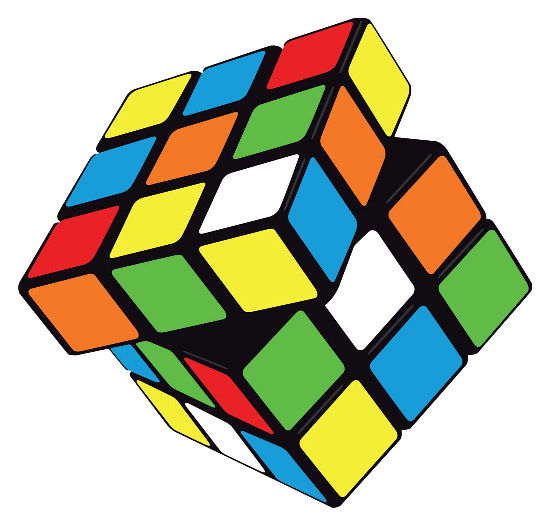
\includegraphics[width=0.15\linewidth]{./vector-rubik-s-cube.eps}};
  Terrible Problem Of Incrementing A Smart Iterator
  \begin{itemize}
    \item Simple usecase\dots
      \begin{center}
        \begin{minipage}{.9\textwidth}
          \begin{minted}{c++}
          auto constexpr isMultipleOf4 = [](int x){ return 0 == x % 4; };
          auto constexpr times2 = [](int x){
              std::cout << "transforming " << x << std::endl;
              return 2*x;
          };
          auto v = rv::iota(1,6) | rv::transform(times2)
                                 | rv::filter(isMultipleOf4);
          for (auto i : v) {/* $\text{to trigger the computation}$ */}
          \end{minted}
        \end{minipage}
      \end{center}
      \vfill
    \item<2-> What's the output?
  \end{itemize}
\end{frame}

\begin{frame}[fragile]{TPOIASI}
  \tikz [remember picture,overlay]
    \node[anchor=north east] at
        (current page.north east)
        {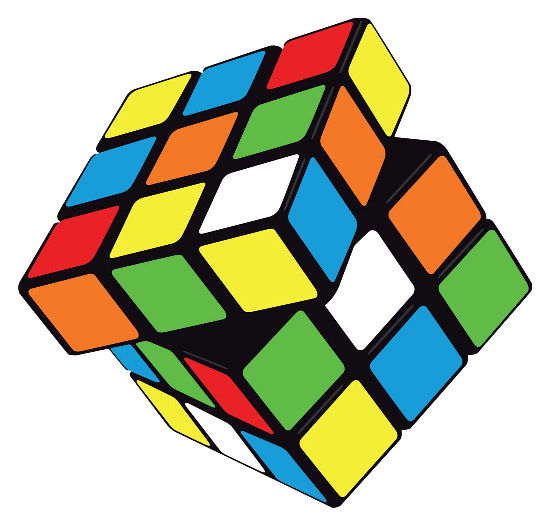
\includegraphics[width=0.15\linewidth]{./vector-rubik-s-cube.eps}};
  \begin{itemize}
    \item<+-> Here it is:
      \begin{center}
        \begin{minted}[mathescape, escapeinside=\#\#]{text}
        transforming 1
        transforming 2
        transforming 2 #$\leftarrow \text{duplicate!}$#
        transforming 3
        transforming 4
        transforming 4 #$\leftarrow \text{duplicate!}$#
        transforming 5
        \end{minted}
      \end{center}
    \item<+-> Why? Long story short:
      \begin{itemize}
        \item \cpp{filter}'s \cpp{operator++} calls \cpp{transform}'s \cpp{operator*}
        \item \cpp{filter}'s \cpp{operator*} calls, again, \cpp{transform}'s \cpp{operator*}
      \end{itemize}
    \item<+-> Solution: caching the result of the \cpp{transform}
      \begin{center}
        \begin{minipage}{.9\textwidth}
          \begin{minted}{c++}
          #include <range/v3/view/cache1.hpp>
          auto v = rv::iota(1,6) | rv::transform(times2)
                                 | rv::cache1
                                 | rv::filter(isMultipleOf4);
          \end{minted}
        \end{minipage}
      \end{center}
  \end{itemize}
\end{frame}

\begin{frame}[fragile]{Meet Miss Hana}
  \tikz [remember picture,overlay]
  \node[anchor=north east] at
  (current page.north east)
  {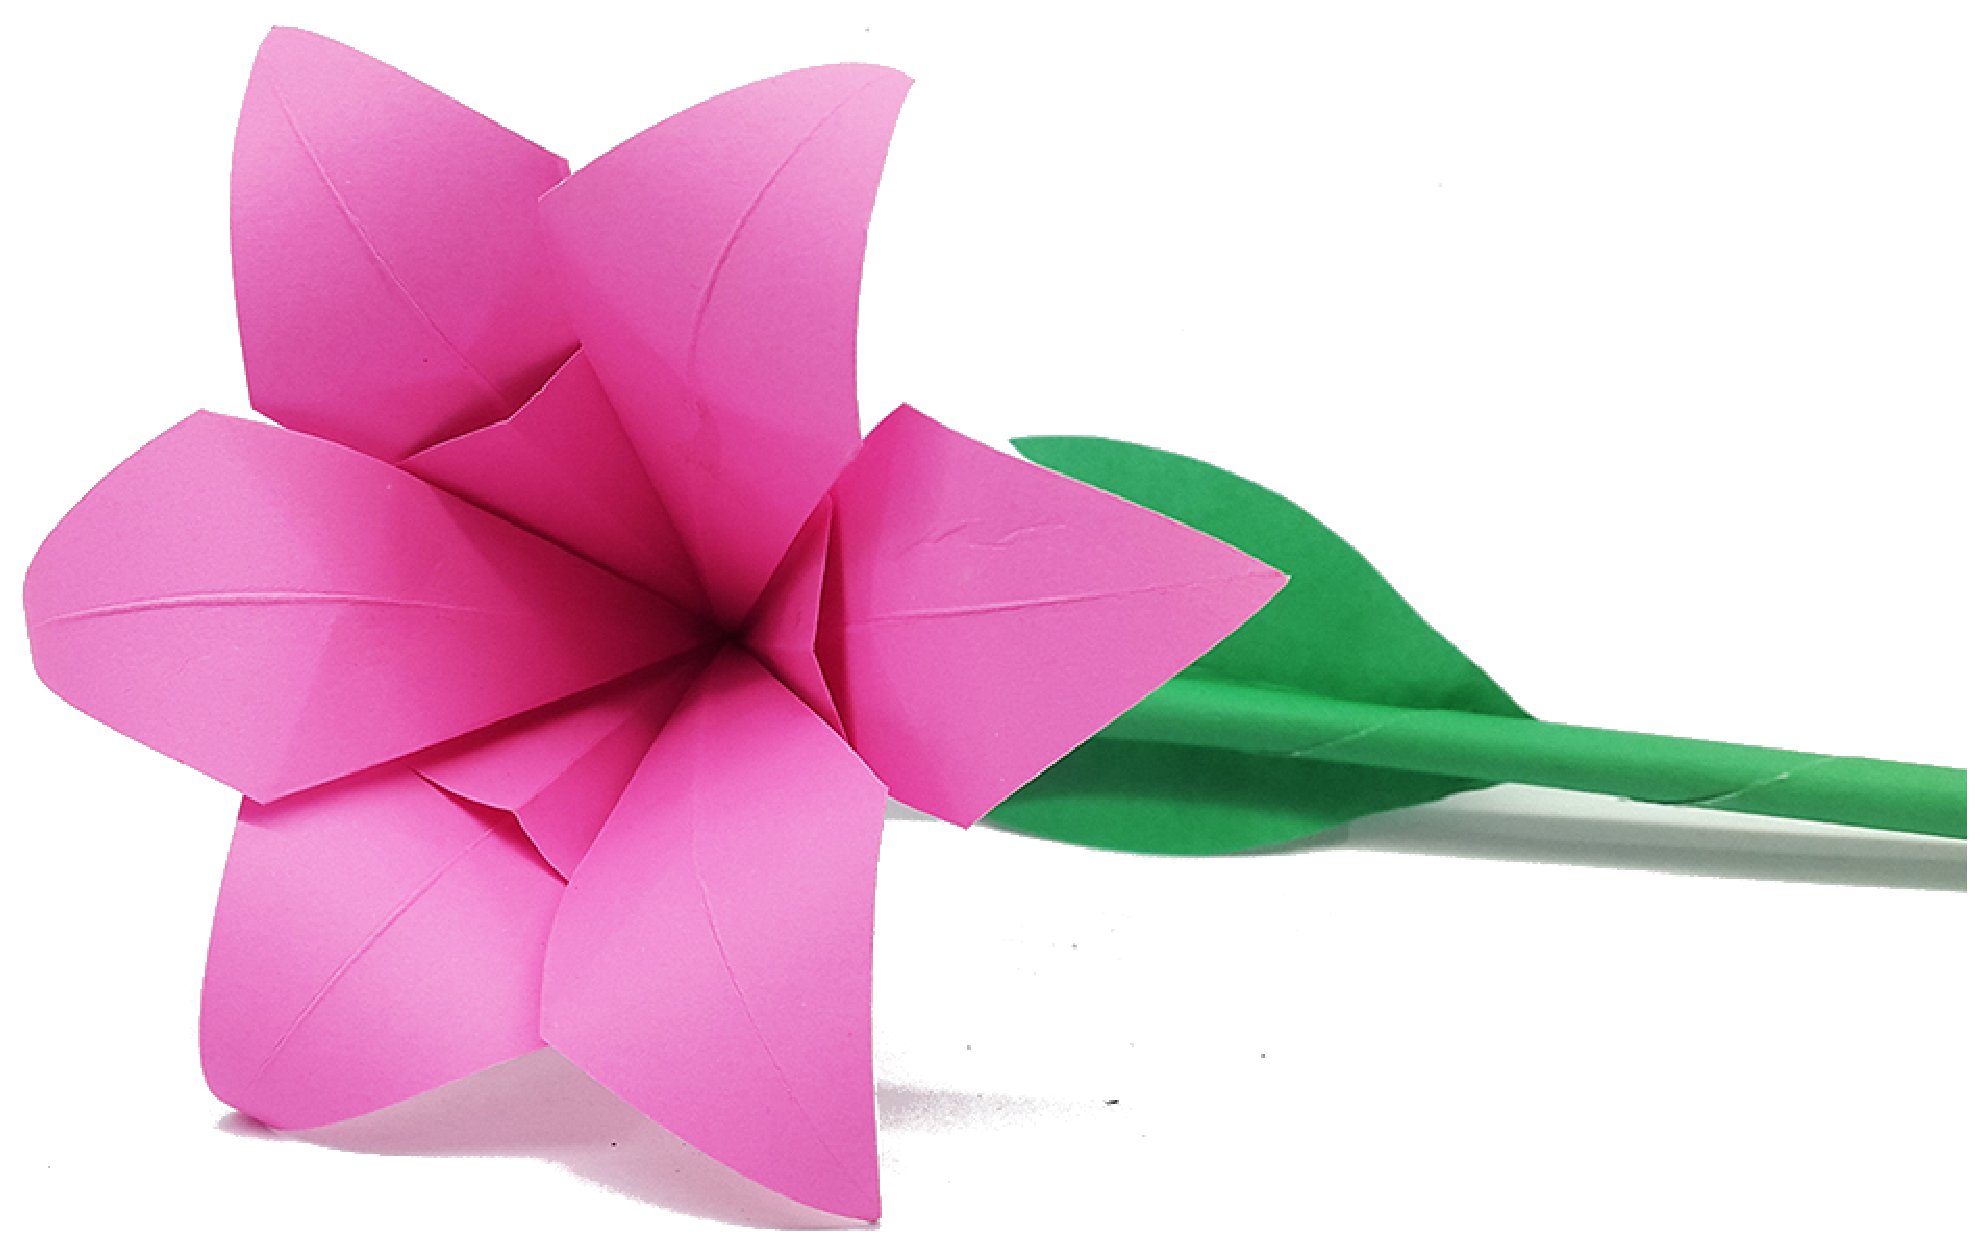
\includegraphics[width=0.2\linewidth]{./How+to+make+lily+Paper+Flower+-+Origami+Flowers+for+Beginners.eps}};
  \begin{itemize}
    \item<+-> The Hana way of \cpp{transform}ing
      \begin{center}
        \begin{minipage}{.9\textwidth}
          \begin{minted}{c++}
          #include <boost/hana/transform.hpp>
          std::vector<int> v = rv::iota(1)
                             | rv::take(10)
                             | r::to_vector;

          auto w = hana::transform(v, times3); // $\text{flipped}$ fmap
          \end{minted}
        \end{minipage}
      \end{center}
      \vfill
    \item<+-> \dots hmmm\dots actually to get the above work, we have to copy
      the \verb|Functor| instance of \cpp{std::vector} from
      \begin{center}
        \begin{minipage}{.9\textwidth}
          \begin{minted}{c++}
          #include <boost/hana/ext/std/vector.hpp>
          \end{minted}
        \end{minipage}
      \end{center}
      which is commented out (Jason Rice on Gitter: \textit{\guillemotleft{} I can only guess it is unfinished. Maybe it needed more tests.\guillemotright})
    \item<+-> What about \verb|Applicative| and \verb|Monad|, by the way? \dots
  \end{itemize}
\end{frame}

\begin{frame}[fragile]{Meet Miss Hana}
  \tikz [remember picture,overlay]
  \node[anchor=north east] at
  (current page.north east)
  {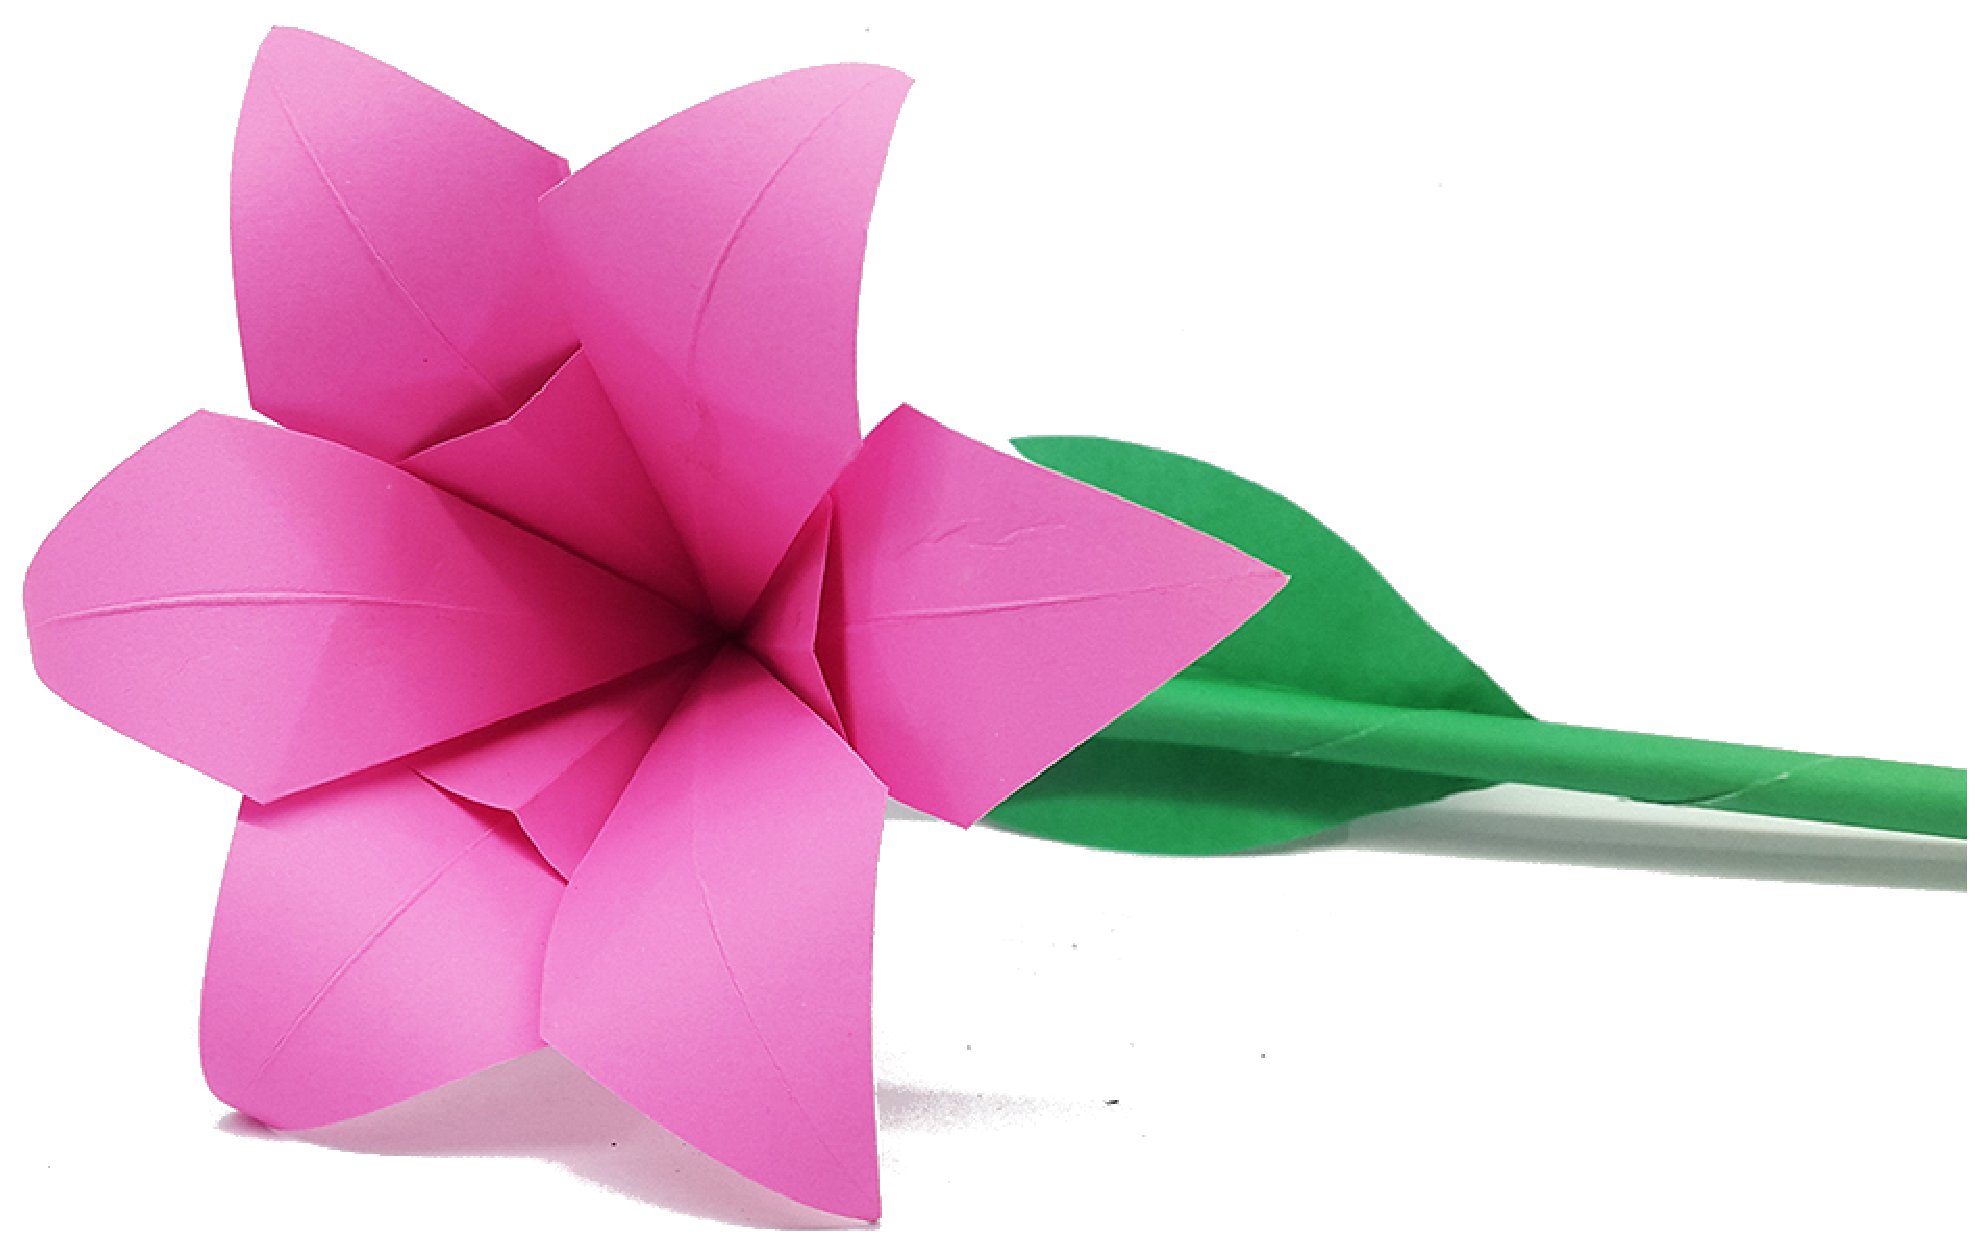
\includegraphics[width=0.2\linewidth]{./How+to+make+lily+Paper+Flower+-+Origami+Flowers+for+Beginners.eps}};
  \begin{itemize}
    \item<+-> What about \verb|Applicative| for \cpp{std::vector}?
    \item<+-> Haskell's \haskell{pure} $\approx$ \cpp{std::vector}'s constructor,
    \item<+-> Haskell's \haskell{(<*>)} $\approx$ ???
    \item<+-> We have a problem. How do we put different functions (with ``only'' the signature in common) into a \cpp{std::vector}?
    \item<+-> Honestly, I have no idea, but the following topics come to my mind:
      \begin{itemize}
        \item type erasure
        \item \cpp{std::function} (does it use type erasure?\dots)
      \end{itemize}
  \end{itemize}
\end{frame}

\begin{frame}[fragile]{More difficult}
  \tikz [remember picture,overlay]
    \node[anchor=north east] at
        (current page.north east)
        {
\includegraphics[width=0.15\linewidth]{./Origami-Jedi-Master-Yoda-1024x576.eps}};
  \begin{itemize}
    \item<+-> Let's take a simple list of lists

      \begin{center}
        \begin{minipage}{.9\textwidth}
          \begin{minted}{haskell}
      xss :: [[Int]]
      xss = [[1,2,3],[4],[5,6]]
          \end{minted}
        \end{minipage}
      \end{center}

    \item<+-> How do we map a function, e.g. \haskell{(+3)}, on it?

    \item<+-> Simple, we use \verb|fmap . fmap|!

      \begin{center}
        \begin{minipage}{.9\textwidth}
          \begin{minted}{haskell}
          yss = (fmap . fmap) (+3) xss
          yss == [[4,5,6],[7],[8,9]]
          \end{minted}
        \end{minipage}
      \end{center}
  \end{itemize}
\end{frame}

\begin{frame}[fragile]{More difficult}
  \tikz [remember picture,overlay]
    \node[anchor=north east] at
        (current page.north east)
        {
\includegraphics[width=0.15\linewidth]{./Origami-Jedi-Master-Yoda-1024x576.eps}};

  What do we need for ``this'' syntax to do the same in C++?

  \begin{center}
    \begin{minipage}{.9\textwidth}
      \begin{minted}{haskell}
      (fmap . fmap) (+3) xss
      \end{minted}
    \end{minipage}
  \end{center}
  Remember that
  \begin{center}
    \begin{minipage}{.9\textwidth}
      \begin{minted}{haskell}
      fmap :: (a -> b) -> f a -> f b
      \end{minted}
    \end{minipage}
  \end{center}
  right \haskell{fmap} gets \haskell{a -> b} and feeds
  \haskell{f a -> f b} to left \haskell{fmap}.
  \vfill
  Therefore we need:
  \begin{itemize}
    \item<2-> an \verb|fmap|-like function,
    \item<3-> since we do have \verb|hana::transform|, we need also a \verb|flip| function,
    \item<4-> a \haskell{(.)}-like operator for function composition,
    \item<5-> currying to appropriately compose non-unary functions (such as \verb|fmap|).
  \end{itemize}

\end{frame}

\begin{frame}[fragile]{Hana to the rescue!}
  \tikz [remember picture,overlay]
    \node[anchor=north east] at
        (current page.north east)
        {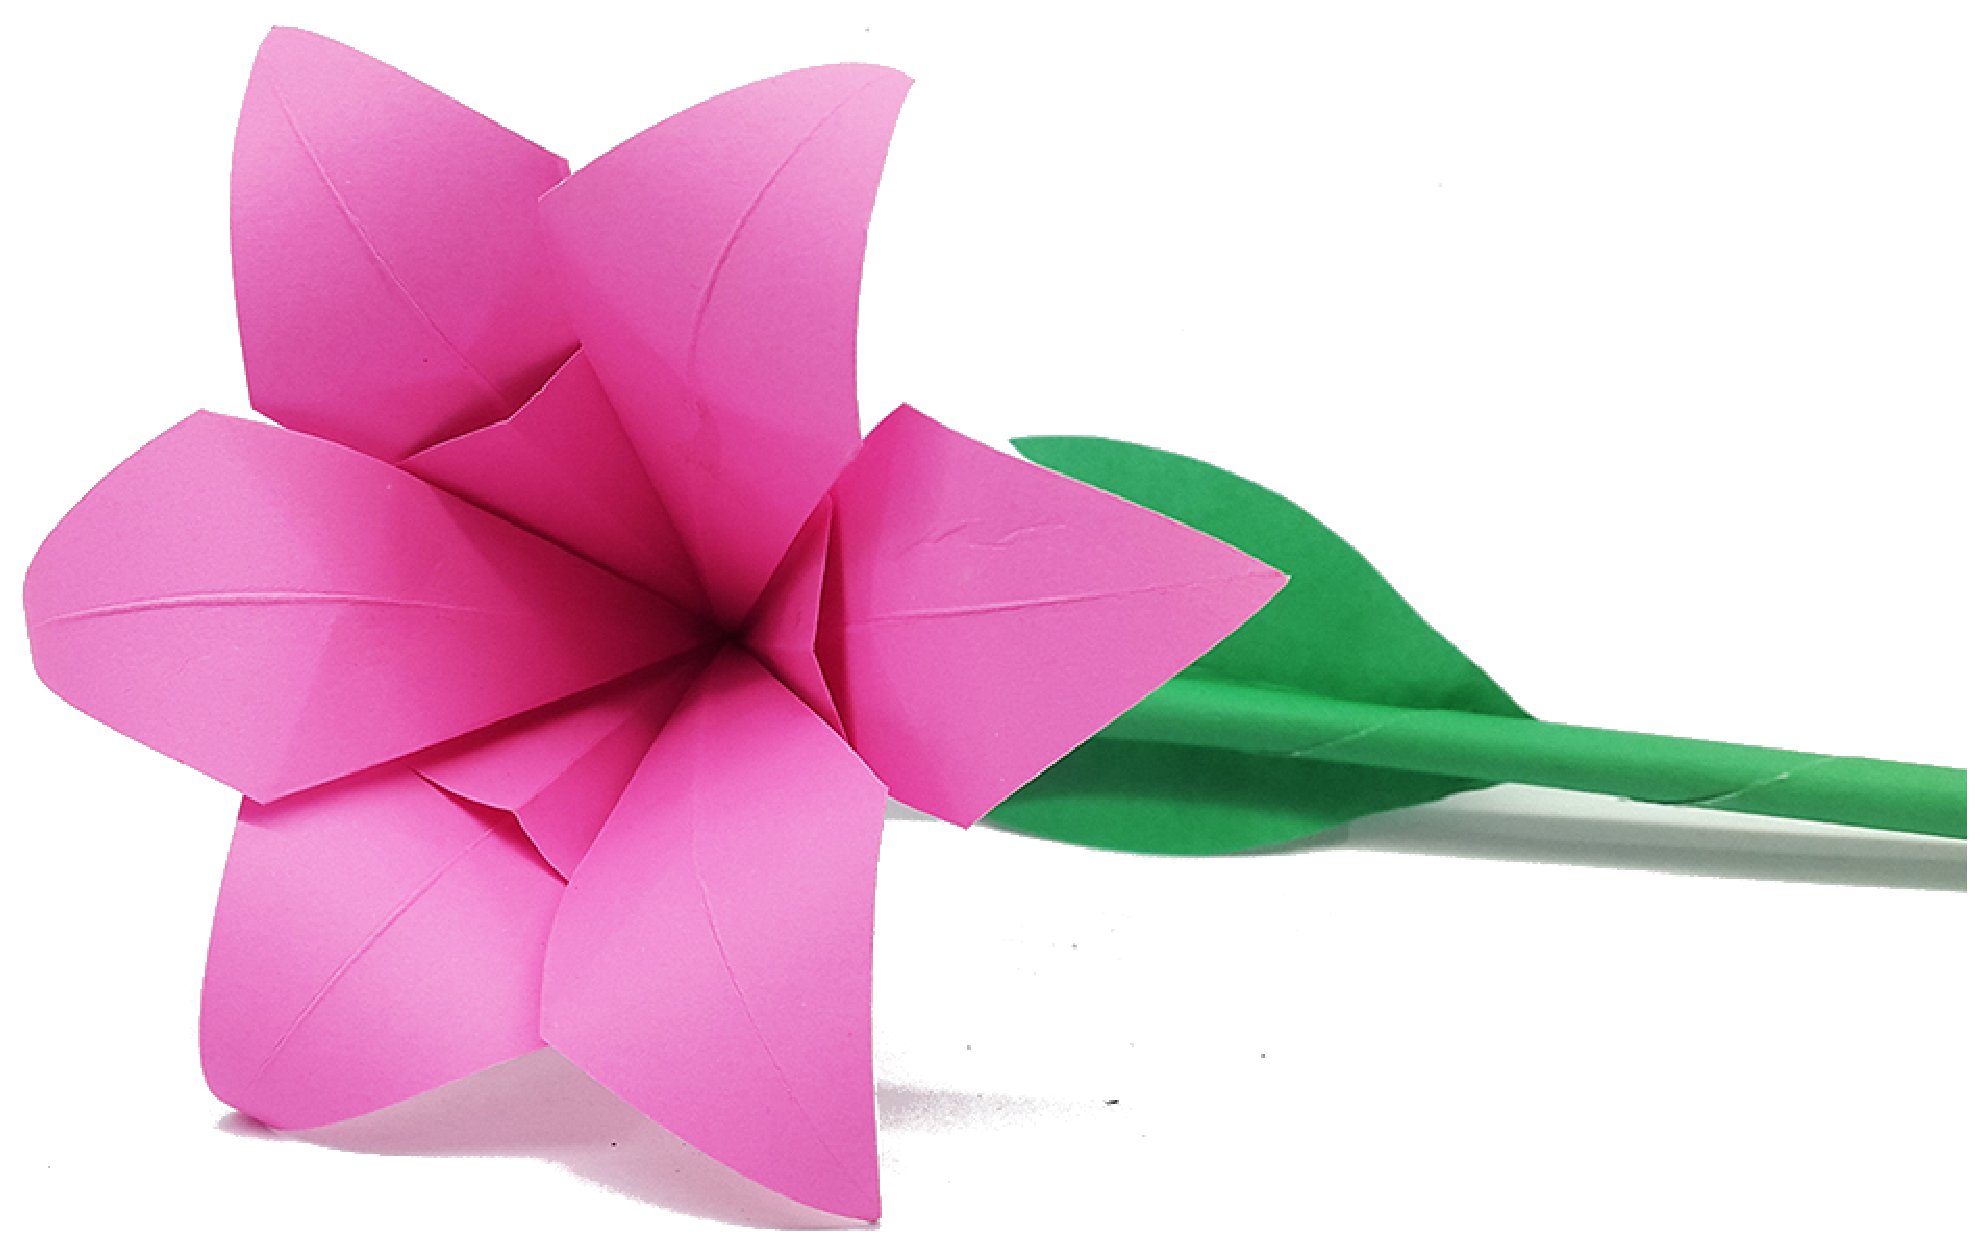
\includegraphics[width=0.2\linewidth]{./How+to+make+lily+Paper+Flower+-+Origami+Flowers+for+Beginners.eps}};

  Needs:
  \begin{itemize}
    \item<2-> an \verb|fmap|-like function,
    \item<4-> since we do have \verb|hana::transform|, we need also a \verb|flip| function,
    \item<6-> a \haskell{(.)}-like operator for function composition,
    \item<8-> currying to appropriately compose non-unary functions (such as \verb|fmap|).
  \end{itemize}
  \vfill
  What does Boost.Hana offer of what we need?
  \begin{itemize}
    \item<3-> \cpp{#include <boost/hana/transform.hpp>}
    \item<5-> \cpp{#include <boost/hana/functional/flip.hpp>}
    \item<7-> \cpp{#include <boost/hana/functional/compose.hpp>}
    \item<9-> \cpp{#include <boost/hana/functional/curry.hpp>}
  \end{itemize}
  \vfill
  \onslide<10->{Simply all!}
\end{frame}

\begin{frame}[fragile]{Hana to the rescue!}
  \tikz [remember picture,overlay]
    \node[anchor=north east] at
        (current page.north east)
        {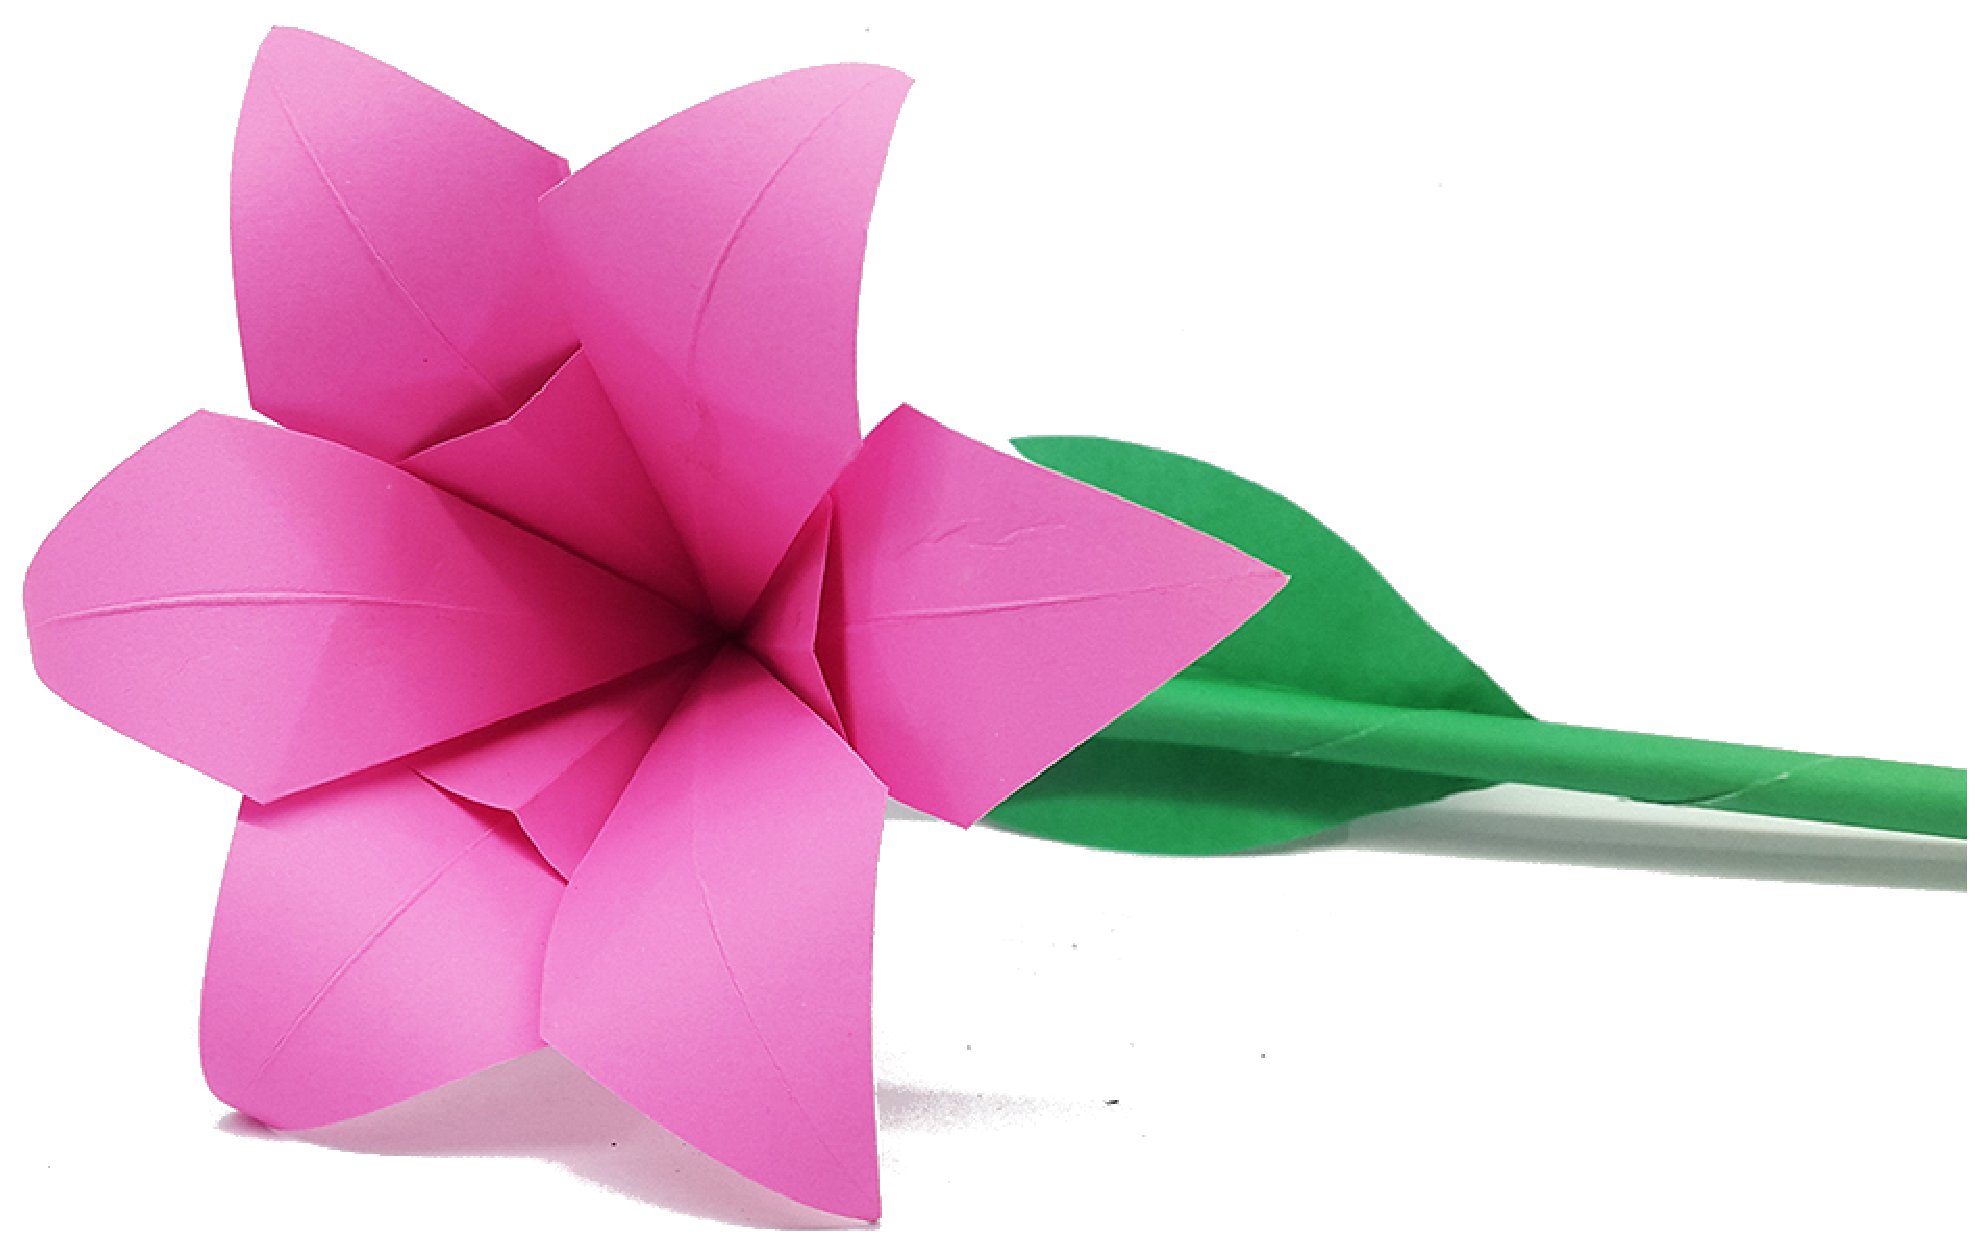
\includegraphics[width=0.2\linewidth]{./How+to+make+lily+Paper+Flower+-+Origami+Flowers+for+Beginners.eps}};
  \begin{itemize}
    \item<+-> Natural solution: imitate Haskell's \haskell{fmap}
      \begin{center}
        \begin{minipage}{.9\textwidth}
          \begin{minted}{c++}
          using namespace boost::hana;
          std::vector<std::vector<int>> xss{{1,2,3},{4},{5,6}};

          auto constexpr fmap = curry<2>(flip(transform));
          auto yss = compose(fmap,fmap)(plus3)(xss);
          // compose(f, g)(x, y...) == f(g(x), y...)
          \end{minted}
        \end{minipage}
      \end{center}
      \vfill
    \item<+-> Actually, \cpp{on} is more powerful and nicer
      \begin{center}
        \begin{minipage}{.9\textwidth}
          \begin{minted}{c++}
          #include <boost/hana/functional/on.hpp>
          auto yss = (fmap ^on^ fmap)(plus3)(xss);
          // on(f, g)(x...) == f(g(x)...)
          \end{minted}
        \end{minipage}
      \end{center}
      \vfill
    \item<+-> Compare with Haskell:
      \begin{center}
        \begin{minipage}{.9\textwidth}
          \begin{minted}{haskell}
        (fmap . fmap) (+3) xss
          \end{minted}
        \end{minipage}
      \end{center}
  \end{itemize}
\end{frame}

\begin{frame}[fragile]{More from Hana}
  \tikz [remember picture,overlay]
    \node[anchor=north east] at
        (current page.north east)
        {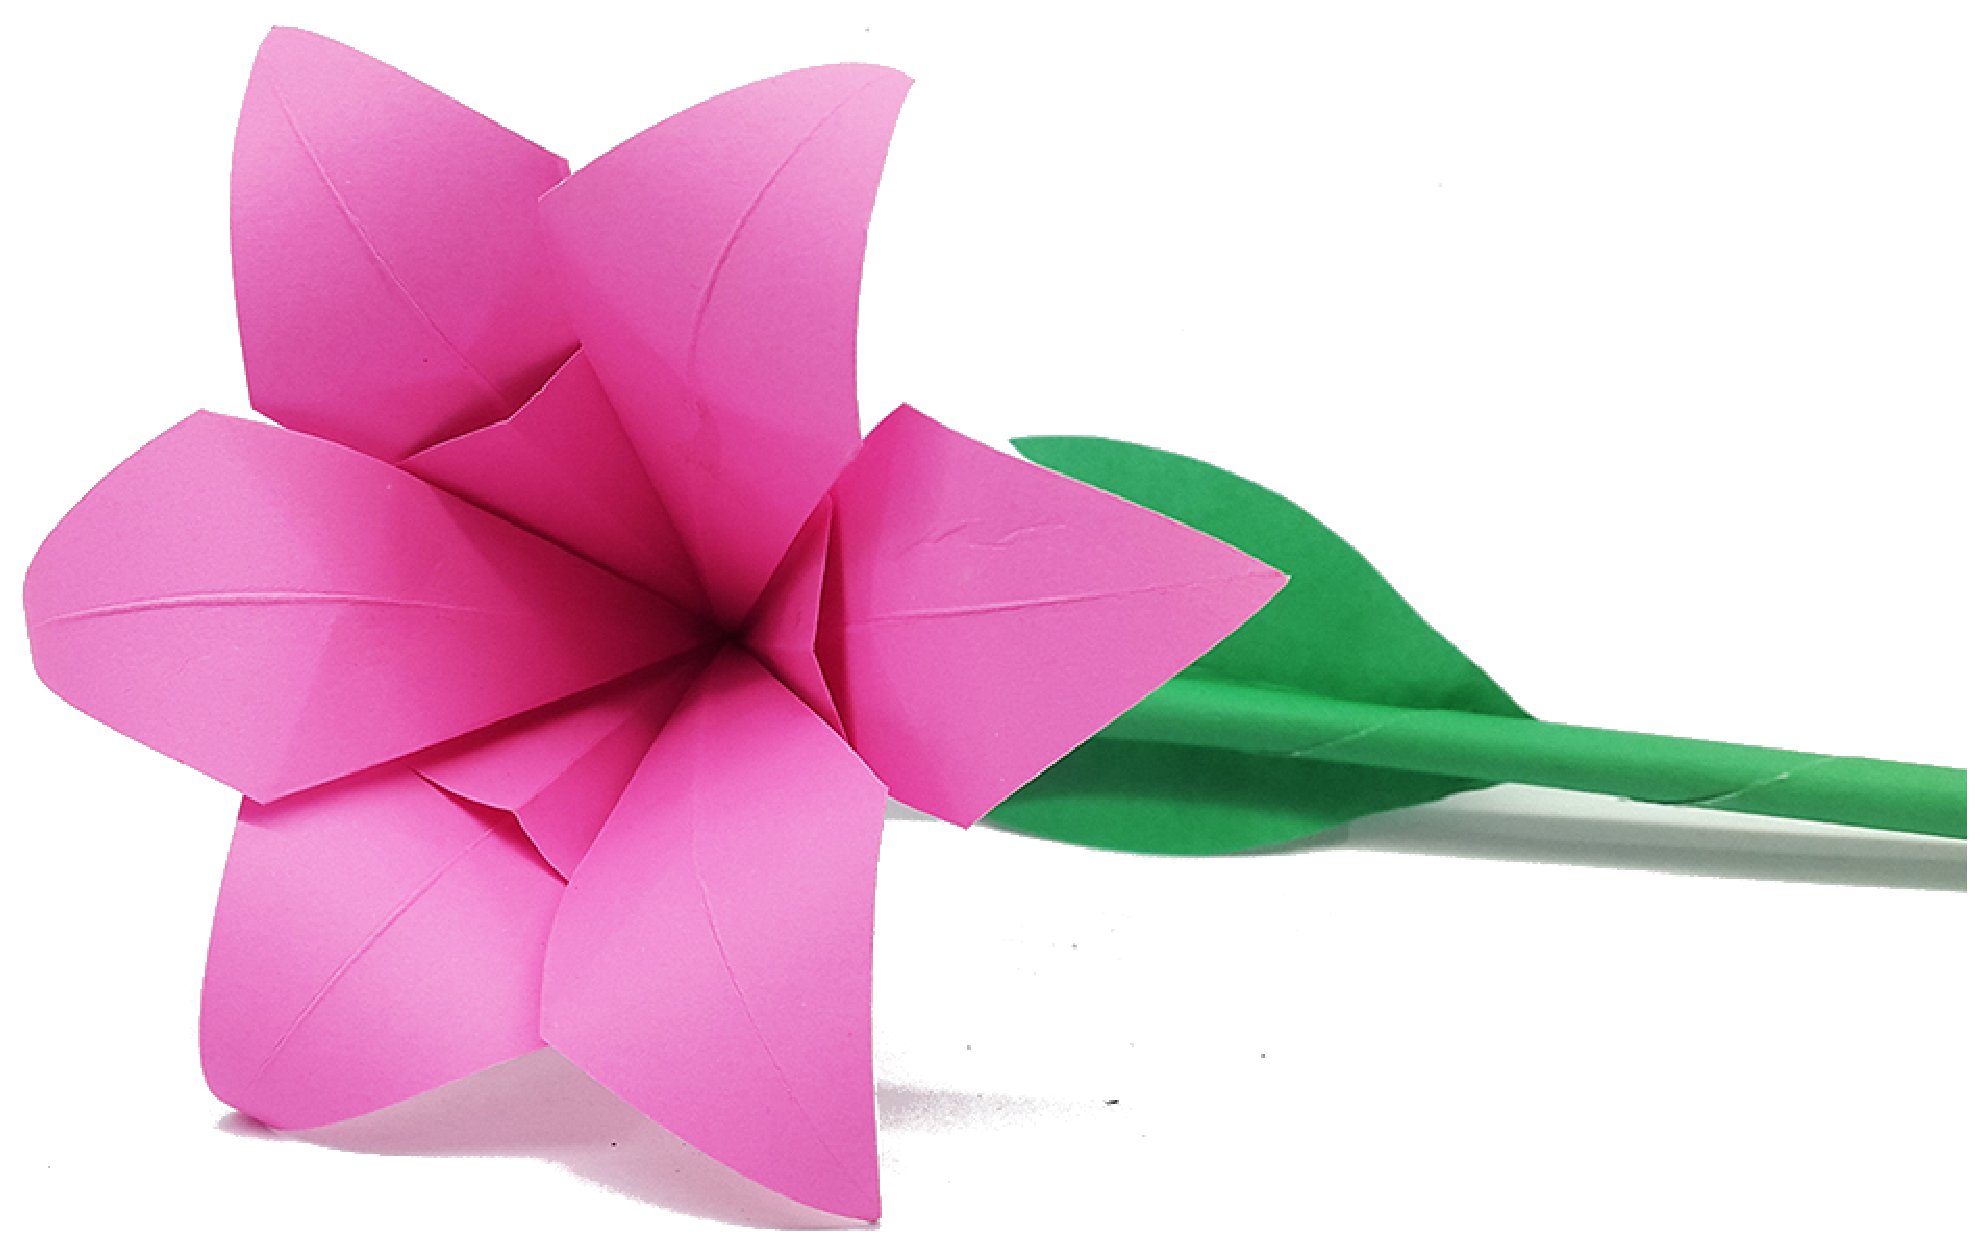
\includegraphics[width=0.2\linewidth]{./How+to+make+lily+Paper+Flower+-+Origami+Flowers+for+Beginners.eps}};
  Hana also offers partial function application:
  \begin{center}
    \begin{minipage}{.9\textwidth}
      \begin{minted}{c++}
      #include <boost/hana/functional/partial.hpp>
      #include <boost/hana/functional/reverse_partial.hpp>
      \end{minted}
    \end{minipage}
  \end{center}
  so these
  \begin{center}
    \begin{minipage}{.9\textwidth}
      \begin{minted}{c++}
      auto constexpr plus3 = [](auto x){ return x + 3; };
      auto divAsDoubles = [](int x, int y){
        return (double)x / y;
      };
      auto r12 = rv::zip_with(divAsDoubles, r1, r2);
      \end{minted}
    \end{minipage}
  \end{center}
  can be rewritten as this
  \begin{center}
    \begin{minipage}{.9\textwidth}
      \begin{minted}{c++}
      auto constexpr plus3 = partial(std::plus<>{}, 3);
      auto constexpr div = std::divides<>{};
      auto constexpr mult = curry<2>(std::multiplies<>{});
      auto r12 = rv::zip_with(div ^on^ mult(1.0), r1, r2);
      \end{minted}
    \end{minipage}
  \end{center}
\end{frame}

\begin{frame}{}
  \begin{center}
    \vfill
    \huge I hope you enjoyed
    \vfill
    \Huge Thank you!
    \vfill
  \end{center}
\end{frame}

\end{document}
